\section{Обчислювальна складність}

\vspace{-\baselineskip}

\subsection{Повний перебір}

Для якісної реконструкції потрібно мати хоча б $20$ параметрів.
Якщо множина значень кожного параметру складається з двох елементів
$\left\{ -1, +1 \right\}$,
потрібно перебрати $2^{20} \approx 10^6$ різних наборів.
Якщо генерація одного обличчя потребує одну соту долю секунди,
перебрати $10^6$ значень вдасться за три години.
При використанні трьох значень $\left\{ -1, 0, +1 \right\}$
отримаємо рік роботи на $3^{20} \approx 3 \cdot 10^9$ векторів $x$.

Зважаючи на те,
що насправді потрібно знати значення параметрів хоча б до цілої частини,
а їх значення знаходяться в проміжку
$\left[ -3; +3 \right]$ за правилом $3 \cdot \sigma$,
стає зрозуміло, що на практиці цей метод використовувати не вийде,
бо $20$ параметрів, кожен з яких приймає $7$ різних значень,
потрібно підбирати десять мільярдів років
($7^{20} \approx 8 \cdot 10^{16}$ різних моделей).

\subsection{Метод Монте-Карло}

Розрахуємо відношення ймовірностей \eqref{eq:monte-carlo:source} для облич,
що відрізняються в одному пікселі на $1$ (мінімальна різниця кольорів)
\begin{equation*}
  \frac{\mathbb{P}_{+1}}{\mathbb{P}_{0}}
  = \frac
    {\exp\left\{- \Sigma - \frac{\left( t_i - f_i \pm 1 \right)^2}{2 \cdot \sigma_t^2}\right\}}
    {\exp\left\{- \Sigma - \frac{\left( t_i \mp f_i \right)^2}{2 \cdot \sigma_t^2}\right\}}
  = \exp{\left\{ \frac{2 \cdot \left( t_i \mp f_i \right) + 1}{2 \cdot \sigma_t^2} \right\}}.
\end{equation*}
Якщо дисперсія дорівнює $1$, маємо
\begin{equation*}
  \frac{\mathbb{P}_{+1}}{\mathbb{P}_{0}}
  = \exp{\left\{ t_i \mp f_i + \frac{1}{2} \right\}}.
\end{equation*}
Оскільки в даному випадку розглядаються цілочисельні зміни кольорів,
модуль показника не може бути меншим за $0.5$.
Мінімальне відношення між ймовірностями двох різних облич
становить $\sqrt{e} \approx 1.7$.
Зазвичай різниця між двома моделями помітна на око,
бо немає сенсу обирати таку точність, яку людина не буде помічати.
З кожним навмання обраним набором параметрів
різниця квадратів змінюється на досить помітне число.
Якщо $10$ пікселів змінять інтенсивність на $2$ одиниці,
ймовірність може не змінитися,
якщо кольори будуть знаходитися за одиницю до та після реального кольору.
Несиметрична зміна кольору на $2$ одиниці в $10$ пікселях призведе
до відношення ймовірностей $e^{-10} \approx 2 \cdot 10^{-9}$.
Навіть такі непомітні зміни призведуть до того,
що одна ймовірність буде більшою за іншу в два мільярди разів,
а їх середнє буде повністю складатися з більшого доданку.

На практиці виявилося,
що інтегрування методом Монте-Карло
для розв'язку задачі з квадратичною функцією витрат~---~задача неможлива.
Різниця ймовірностей між навмання обраними моделями обличчя неймовірно велика,
тому метод перетворювався на пошук глобального максимуму функції
шляхом генерації випадкових параметрів.
Такий підхід може бути доцільним
для генерації початкових умов алгоритму локальної оптимізації,
проте без цієї модифікації випадкова генерація моделей
не має ніяких переваг над іншими методами.

\subsection{Баєсова стратегія}

Субоптимальна баєсова стратегія,
що є розв'язком системи \eqref{eq:problem:bayesian:suboptimal}
\begin{equation*}
  \begin{cases}
    c \to \min, \\
    R_{\theta}\left( q \right)
      - R_{\theta}\left( q^{\theta} \right) < c,
    \qquad \forall \theta \in \Theta,
  \end{cases}
\end{equation*}
де $q$ за теоремою про дихотомію має вигляд \cite{schlezinger:2013}
\begin{equation*}
  \begin{cases}
    \sum\limits_{\theta \in \Theta} \tau\left( \theta \right) = 1, \\
    \tau\left( \theta \right) \ge 0, \qquad \forall \theta \in \Theta, \\
    q = \argmin\limits_{q \in Q} \sum\limits_{\theta \in \Theta}
      \tau\left( \theta \right) \cdot R_{\theta}\left( q \right),
  \end{cases}
\end{equation*}
потребує розрахунку ризиків оптимальних стратегій
\eqref{eq:problem:bayesian:optimal}
\begin{equation*}
  q^{\theta}
  = \argmin\limits_{q \in Q} R_{\theta}\left( q \right)
\end{equation*}
для кожного $\theta$.

Дискретизуємо простір параметрів моделі так,
щоб кожен параметр приймав лише по $7$ цілих значень
з проміжку $\left[ -3; +3 \right]$,
візьмемо бінарну функцію витрат та введемо припущення,
що локальний екстремум співпадає з глобальним.
Розрахунок ризику~---~це інтегрування по множині можливих параметрів моделі.
У попередньому підпункті було вказано,
що навіть візуалізувати необхідну кількість різних облич неможливо,
але дане завдання ускладнюється необхідністю
багатократного запуску алгоритму локальної оптимізації.
Припустимо, що було взято дуже мало параметрів~--~наприклад, два.
Отримаємо лише $49$ різних облич.
При фіксованому фоні, рівні шуму, освітленні, повороті та розмірі обличчя
можна легко підібрати обидва параметри повним перебором.

Наступною проблемою є множина можливих параметрів.
Візьмемо кути нахилу від $-\frac{\pi}{2}$ до $+\frac{\pi}{2}$.
Якщо використовувати досить помітну зміну кута $\frac{\pi}{6}$
(рис.~\ref{fig:practice:angles}),
отримаємо $6$ різних позицій для кожного кута Ейлера.
Оскільки їх $3$, доведеться вести розрахунки для $216$ різних поворотів.
\begin{figure}[h]
  \centering
  \begin{subfigure}[b]{0.3\textwidth}
    \centering
    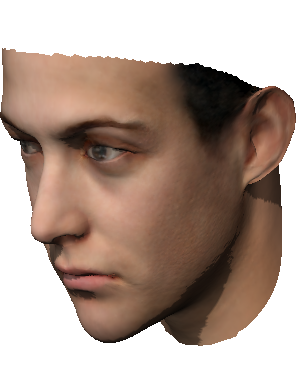
\includegraphics[width=\textwidth]{images/face_rotated_1}
    \caption{Початкове положення}
  \end{subfigure}
  \begin{subfigure}[b]{0.3\textwidth}
    \centering
    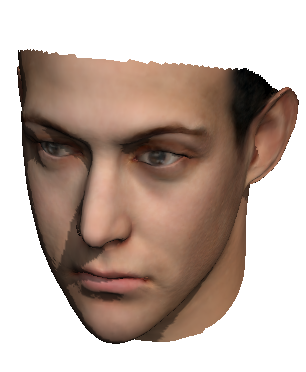
\includegraphics[width=\textwidth]{images/face_rotated_2}
    \caption{Поворіт вбік}
  \end{subfigure}
  \begin{subfigure}[b]{0.3\textwidth}
    \centering
    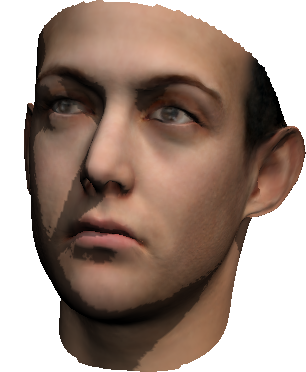
\includegraphics[width=\textwidth]{images/face_rotated_3}
    \caption{Поворіт вбік и вгору}
  \end{subfigure}
  \caption{Повороти обличчя на $30^{\circ}$ по різним осям}
  \label{fig:practice:angles}
\end{figure}

Освітлення є одним з важливіших параметрів,
бо саме воно формує зовнішній вигляд обличчя,
і може як допомогти, так і ввести в оману.
Положення джерела світла описується лише двома кутами,
проте діапазон можливих значень повинен бути ширше
за можливі значення повороту голови,
бо джерело може світити ззаду, через що модель буде майже повністю темна.
З кроком $\frac{\pi}{6}$
(рис.~\ref{fig:practice:shadows-angles-azimuth}
та рис.~\ref{fig:practice:shadows-angles-zenith})
та значеннями від $-\pi$ до $+\pi$
маємо $12$ значень на кожну компоненту та $144$ загалом.
Також треба мати хоча б $5$ різних значень інтенсивності світла.
\begin{figure}[h]
  \centering
  \begin{subfigure}[b]{0.4\textwidth}
    \centering
    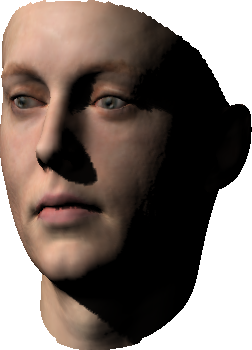
\includegraphics[width=\textwidth]{images/face_shaded_1}
    \caption{Початкове положення}
  \end{subfigure}
  \begin{subfigure}[b]{0.4\textwidth}
    \centering
    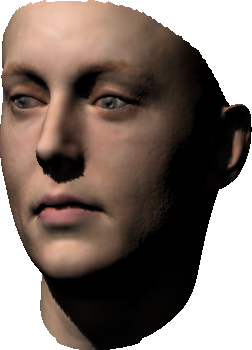
\includegraphics[width=\textwidth]{images/face_shaded_2}
    \caption{Зміна азимутального кута на $30^{\circ}$}
  \end{subfigure}
  \caption{Переміщення джерела світла по азимуту}
  \label{fig:practice:shadows-angles-azimuth}
\end{figure}

\begin{figure}[h]
  \centering
  \begin{subfigure}[b]{0.4\textwidth}
    \centering
    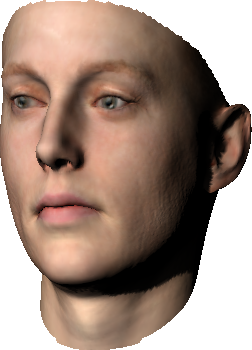
\includegraphics[width=\textwidth]{images/face_shaded_3}
    \caption{Зменшення зенітного кута на $30^{\circ}$}
  \end{subfigure}
  \begin{subfigure}[b]{0.4\textwidth}
    \centering
    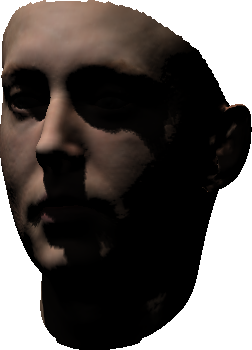
\includegraphics[width=\textwidth]{images/face_shaded_4}
    \caption{Збільшення зенітного кута на $30^{\circ}$}
  \end{subfigure}
  \caption{Переміщення джерела світла по зеніту}
  \label{fig:practice:shadows-angles-zenith}
\end{figure}

Бачимо, що навіть без врахування фону, переміщення і шуму потрібно перебрати
$144 \cdot 5 \cdot 216 = 155520 \approx 1.5 \cdot 10^{5}$ різних параметрів
для кожного з $49$ облич.
Їх генерація забере $21$ годину.
Для кожного згенерованого обличчя потрібно запустити процедуру оптимізації,
щоб визначити точність роботи алгоритму за даних параметрів.
Якщо використати одну ітерацію покомпонентного спуску,
знадобиться перебрати лише по $14$ облич для кожного зображення,
що потребує $12$ діб роботи на одному комп'ютері,
що візуалізує одну модель за одну соту долю секунди.

На рисунку~\ref{fig:practice:angles} видно,
що обрана зміна кута повороту дуже помітна,
проте з рисунку~\ref{fig:practice:shadows-angles-zenith} помітно,
що для зенітного кута освітлення
обраний крок дискретизації є досіть значним,
а чим зеніт ближчий до прямого кута,
тим значніший азімутний поворіт.
Обрана роздільна сітка не підходить
і потрібно ще зменшити крок зміни положення джерела освітлення.

Якщо грамотно поставити експеримент та паралельно обчислювати значення ризиків,
то для моделей з дуже малою кількістю параметрів за реальний час можна зібрати дані
для одної ітерації розв'язку задачі \eqref{eq:problem:bayesian:suboptimal}.
Хоча вказаний час не є прийнятним для кількох десятків кроків
алгоритму пошуку субоптимальної стратегії,
зібрані дані вкажуть максимальну якість розпізнавання,
на яку можна сподіватися при певних значеннях невідомих параметрів,
що в свою чергу можна використовувати як
відомості про обмеження на умови експлуатації системи реконструкції.

На даний момент цей спосіб являє собою виключно теоретичний інтерес,
проте з розвитком комп'ютерної техніки у найближчі роки можна буде
провести даний експеримент з більшою точністю за прийнятний час та ціну,
що дозволить використовувати субоптимальну стратегію на практиці.
